% !TEX root = ../../../main.tex

\toggletrue{image}
\toggletrue{imagehover}
\chapterimage{division_notation}
\chapterimagetitle{\uppercase{Division Notation}}
\chapterimageurl{https://xkcd.com/2687/}
\chapterimagehover{Science tip: Scientists hardly ever use the two-dot division sign, and when they do it often doesn't even mean division, but they still get REALLY mad when you repurpose it to write stuff like SALE! ALL SHOES 30÷ OFF!}

\chapter{Ganzzahlige Division}
\label{chapter-ganzzahlige-division}

% TODO Quelle: https://crypto.ethz.ch/teaching/DM21/ln/DM21_LN_8jk9jkr58uo2kq7mzarv.pdf

Wenn wir mit natürlichen oder ganzen Zahlen arbeiten, dann können wir die ganzzahlige Division mit Rest durchführen. Dieses Verfahren haben Sie vielleicht schon kennengelernt, als Sie noch nicht \say{richtig} dividieren konnten\footnote{Zum Beispiel in der Primarschule.}. Die Lernziele lauten:

\newcommand{\ganzzahligeDivisionLernziele}{
\protect\begin{todolist}
\item Sie führen die ganzzahlige Division durch.
\item Sie berechnen den Rest einer ganzzahligen Division.
\end{todolist}
}

\lernziel{\autoref{chapter-ganzzahlige-division}, \nameref{chapter-ganzzahlige-division}}{\protect\ganzzahligeDivisionLernziele}

\ganzzahligeDivisionLernziele

\section{Rechenschritte}

Wir zeigen die Berechnung der ganzzahligen Division mit Rest an einem Beispiel.

\begin{example}
Wir dividieren ganzzahlig $9$ durch $4$ mit Rest.

\begin{enumerate}
\item Berechne die Division zunächst wie gewöhnlich mit Komma: $9 : 4 = 2,25$
\item Der \textbf{ganzzahlige Anteil} der Division ist die Zahl \say{vor dem Komma}: $2$
\item Den \textbf{Rest} der ganzzahligen Division erhalten wir durch die Multiplikation von Divisor und Nachkommastellen: $4 \cdot 0,25 = 1$
\end{enumerate}

Wir schreiben die Rechnung kompakt wie folgt: $9 : 4 = 2~\text{Rest}~1$. \autoref{figure-ganzzahlige-division-kuchen} zeigt die ganzzahlige Division am Beispiel der \say{Kuchenverteilung}.

\begin{figure}[htb]
	\centering
	\begin{minipage}{0.45\textwidth}
		\centering
		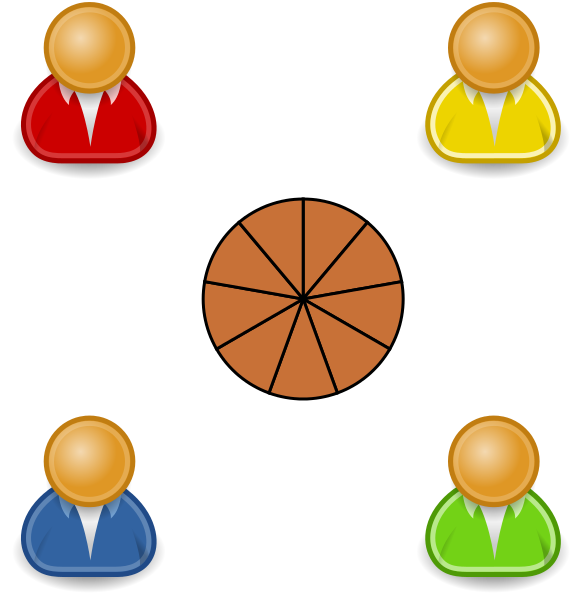
\includegraphics[scale=0.215]{pie_division_1}		
	\end{minipage}
	\hfill
	\begin{minipage}{0.45\textwidth}
		\centering
		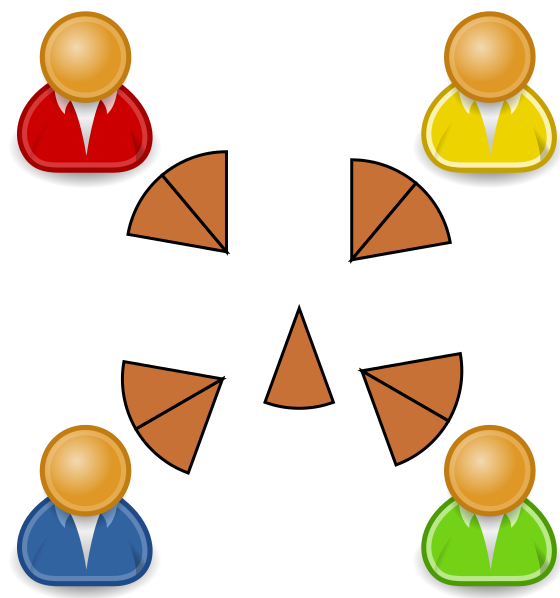
\includegraphics[scale=0.215]{pie_division_2}		
	\end{minipage}
	\caption{Neun Kuchenstücke sollen auf vier Personen verteilt werden. Pro Person gibt es zwei Kuchenstücke und ein Kuchenstück bleibt übrig: $9 : 4 = 2 + 1$ \cite{wiki2012piedivision}.}
	\label{figure-ganzzahlige-division-kuchen}
\end{figure}

\end{example}

\section{Ganzzahlquotient und Modulo}

Manchmal möchten wir nur den Wert der ganzzahligen Division oder den Rest bestimmen. Dafür gibt es separate Rechenoperationen.

\begin{definition}[Ganzzahlquotienten]
Möchten wir eine ganzzahlige Division durchführen und nur den Ganzzahlquotienten bestimmen (\say{den Rest weglassen}), dann verwenden wir dafür $\div$ als Rechensymbol. Wir schreiben für zwei ganze Zahlen somit $a \div b$.	
\end{definition}

\begin{example}
Mit dem Zahlenbeispiel von vorher erhalten wir $9 \div 4 = 2$. 
\end{example}

\begin{definition}[Modulo]
Möchten wir eine ganzzahlige Division durchführen und nur den \textbf{Rest} bestimmen, dann verwenden wir dafür $\bmod$ als Rechensymbol. Wir schreiben für zwei ganze Zahlen somit $a \bmod b$.  Das Rechensymbol $\bmod$ ist eine Abkürzung für \textbf{Modulo-Operator}. Modulo bezeichnet den Rest der ganzzahligen Division.
\end{definition}

\begin{example}
Mit dem Zahlenbeispiel von vorher erhalten wir $9 \bmod 4 = 1$. 
\end{example}

\begin{important}
Der Modulo-Operator ist für die Kryptologie entscheidend. Machen Sie sich unbedingt mit dem Umgang damit vertraut.
\end{important}


\section{Aufgaben}

\begin{enumerate}
	\item Schreiben Sie das Ergebnis der folgenden Berechnungen direkt hinter die Teilaufgabe.

\begin{multicols}{3}
\begin{enumerate}
\item $72 \div 9 = \rule[-0.75mm]{1cm}{.5pt}$
\item $72 \bmod 9 = \rule[-0.75mm]{1cm}{.5pt}$
\item $225 \div 3 = \rule[-0.75mm]{1cm}{.5pt}$
\item $225 \bmod 3 = \rule[-0.75mm]{1cm}{.5pt}$
\item $257 \div 8 = \rule[-0.75mm]{1cm}{.5pt}$
\item $257 \bmod 8 = \rule[-0.75mm]{1cm}{.5pt}$
\item $13 \div 25 = \rule[-0.75mm]{1cm}{.5pt}$
\item $13 \bmod 25 = \rule[-0.75mm]{1cm}{.5pt}$
\item $31 \div 26 = \rule[-0.75mm]{1cm}{.5pt}$
\item $31 \bmod 26 = \rule[-0.75mm]{1cm}{.5pt}$
\item $7 \div 3 = \rule[-0.75mm]{1cm}{.5pt}$
\item $7 \bmod 3 = \rule[-0.75mm]{1cm}{.5pt}$
\item $0 \bmod 2 = \rule[-0.75mm]{1cm}{.5pt}$
\item $1 \bmod 2 = \rule[-0.75mm]{1cm}{.5pt}$
\item $2 \bmod 2 = \rule[-0.75mm]{1cm}{.5pt}$
\item $15 \bmod 7 = \rule[-0.75mm]{1cm}{.5pt}$
\item $24 \bmod 7 = \rule[-0.75mm]{1cm}{.5pt}$
\item $42 \bmod 7 = \rule[-0.75mm]{1cm}{.5pt}$
\end{enumerate}
\end{multicols}

	\item Sei $a$ eine positive, gerade Zahl. Wie lautet das Ergebnis von $a \bmod 2$? Warum?
	
	\fillwithgrid	{1in}
	
	\item Sei $a < b$. Wie lautet das Ergebnis von $a \bmod b$? Begründen Sie Ihre Antwort.
	
	\fillwithgrid	{1in}
	
	\item Was gilt für die Modulorechnung, wenn $x$ ein Teiler von $y$ ist. Nehmen Sie an, dass $x$ und $y$ zwei natürliche, positive Zahlen sind.

	\fillwithgrid	{1in}

\end{enumerate}